\section{Materiales}
\begin{minipage}{0.8\linewidth}
    \begin{multicols}{2}
    \begin{itemize}
        \item Cronómetro digita
        \item Sensor
        \item Medidor de ángulos
        \item Esfera de metal
        \item Sujetador
        \item Núez
        \item Báscula
    \end{itemize}
\end{multicols}
\end{minipage}
\begin{minipage}{0.2\linewidth}
    \begin{figure}[H]
        \centering
        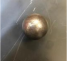
\includegraphics[scale=0.8]{Images/ima1.png}
        \label{fig:ima1}
    \end{figure}
\end{minipage}
\section{Procedimiento}
\begin{minipage}{0.22\linewidth}
    \begin{figure}[H]
        \centering
        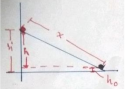
\includegraphics[scale=0.75]{Images/ima2.png}
        \label{fig:ima2}
    \end{figure}
\end{minipage}
\begin{minipage}{0.58\linewidth}
    Apoyada sobre el soporte universal, se colocó una rampa de
longitud x = 1.83m muescada por el centro e inclinada en
un ángulo variable, por la que se rodó una esfera de radio
R = 1.15cm. Al inicio del plano se colocó la paleta iman-
tada del cronómetro y al final se colocó la paleta detectora.
Como se dijo antes,
\end{minipage}
\begin{minipage}{0.2\linewidth}
    \begin{figure}[H]
        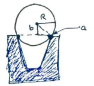
\includegraphics[scale=1]{Images/ima3.png}
        \label{fig:ima3}
    \end{figure}
\end{minipage}
\vspace{-0.7cm}\\
se varió el ángulo del riel para obtener diferentes tiempos al dejar rodar la esfera. Por razones técnicas, se obtuvo la altura real a través de la que
rodó la esfera restando h 0 de h‘, como se aprecia en el diagrama\\
\begin{minipage}{0.4\linewidth}
    \begin{table}[H]
        \centering
        \begin{tabular}{cccc} \hline
            t(s) & h(m)& h\textsubscript{0}(m)& h(m) \\ \hline
1.13&1.10 &0.155 &0.945\\
1.21&1.00 &0.145 &0.855\\
1.24&0.90 &0.140 &0.760\\
1.29&0.85 &0.130 &0.720\\
1.37&0.75 &0.120 &0.630\\
1.58&0.60 &0.100 &0.500\\
1.80&0.45 &0.090 &0.360\\ \hline
        \end{tabular}
    \end{table}
\end{minipage}
\begin{minipage}{0.6\linewidth}
    De las mediciones se obtuvo la información de la tabla, que por método de
regresión logarítmica arrojó la función
\begin{equation}
    y=1.216x^{-2.035}
    \label{eq:min}
\end{equation}
que comparada con la ecuación \ref{eq:h}, se tiene que
\begin{equation}
    \changefontsizes{9pt}
    h=\frac{2(1.83)^2}{9.81} \left(\frac{2(0.0115)^2}{5(0.00006825)^2}+1 \right)t^{-2}= 1.212 t^{-2}
    \label{eq:h2}
\end{equation}
\end{minipage}
\begin{minipage}{0.55\linewidth}
    al igualar las ecuaciones \ref{eq:min} y \ref{eq:h} 
\begin{equation*}
    1.216t^{-2.035} \approx 1.212 t^{-2}.
\end{equation*}
Por lo tanto, se demuestra la validez de la ecuación \ref{eq:h} a través de pruebas experimentales.
\end{minipage}
\begin{minipage}{0.35\linewidth}
    \begin{figure}[H]
        \centering
        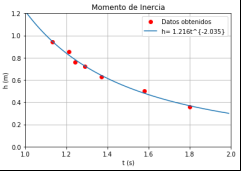
\includegraphics[scale=0.8]{Images/ima4.png}
    \end{figure}
\end{minipage}